% Editable standalone vector figure extracted from spectra.tex.
% Source slide 20; figure 19; native embedded fonts.
% Compile with LuaLaTeX from this directory, or run ../export_figures.py.
\documentclass[tikz,border=0pt]{standalone}
% Shared editable preamble for standalone, Nature-style vector figures.
% Text remains embedded and searchable. This is a house-style target, not a
% claim of acceptance or of satisfying every journal's submission checklist.
\usepackage{fontspec}
\setmainfont{LiberationSans}[
  Path=../../shared/assets/,Extension=.ttf,
  UprightFont=*-Regular,BoldFont=*-Bold,ItalicFont=*-Italic,BoldItalicFont=*-BoldItalic]
\setsansfont{LiberationSans}[
  Path=../../shared/assets/,Extension=.ttf,
  UprightFont=*-Regular,BoldFont=*-Bold,ItalicFont=*-Italic,BoldItalicFont=*-BoldItalic]
\setmonofont{LiberationSans}[
  Path=../../shared/assets/,Extension=.ttf,
  UprightFont=*-Regular,BoldFont=*-Bold,ItalicFont=*-Italic,BoldItalicFont=*-BoldItalic]
\usepackage{unicode-math}
\setmathfont{Latin Modern Math}
\DeclareMathSizes{5.9}{6}{5}{5}
\DeclareMathSizes{6}{6}{5}{5}
\usepackage{tikz}
\usetikzlibrary{arrows.meta,calc,positioning,patterns,decorations.pathreplacing,matrix}
\usepackage{graphicx}
\usepackage{xcolor}
\pagecolor{white}
\definecolor{ink}{HTML}{202020}
\definecolor{paper}{HTML}{FFFFFF}
\definecolor{muted}{HTML}{494949}
\definecolor{line}{HTML}{808080}
\definecolor{soft}{HTML}{F0F0F0}
\hyphenpenalty=10000\exhyphenpenalty=10000
\newcommand{\figurefont}{\sffamily\fontsize{5.9}{7.4}\selectfont}
\newcommand{\figuremathfont}{\sffamily\fontsize{6}{7.5}\selectfont}
\newcommand{\brandmedium}{\bfseries}
\renewcommand{\normalsize}{\figurefont}
\renewcommand{\small}{\figurefont}
\renewcommand{\footnotesize}{\figurefont}
\renewcommand{\scriptsize}{\figurefont}
\renewcommand{\tiny}{\figurefont}
\renewcommand{\large}{\figurefont}
\renewcommand{\Large}{\figurefont}
\renewcommand{\LARGE}{\figurefont}
\renewcommand{\huge}{\figurefont}
\renewcommand{\Huge}{\figurefont}
\tikzset{
  every path/.style={line width=.55pt},
  every node/.style={font=\figurefont,text=ink},
  arr/.style={-{Latex[length=1.5mm,width=1mm]},line width=.55pt,draw=ink},
  thinarr/.style={-{Latex[length=1.3mm,width=.9mm]},line width=.55pt,draw=ink},
  box/.style={draw=ink,line width=.55pt,fill=white,minimum height=.85cm,align=center,inner sep=3pt},
  ghost/.style={draw=muted,dashed,fill=soft},
  tag/.style={font=\figurefont,text=muted},
  equ/.style={font=\figuremathfont},
  small/.style={font=\figurefont},
  body/.style={font=\figurefont},
  tinytext/.style={font=\figurefont}
}
\newcommand{\txt}[4]{\node[anchor=north west,align=left,text width=#3cm] at (#1,#2) {#4};}
\newcommand{\smalltxt}[4]{\node[anchor=north west,align=left,text width=#3cm,small] at (#1,#2) {#4};}
\newcommand{\eqn}[4][6]{\node[anchor=north west,font=\figuremathfont] at (#2,#3) {$\displaystyle #4$};}
\newcommand{\diagramblock}[5]{\node[box,minimum width=#3cm,text width=#3cm,minimum height=#4cm] at (#1,#2) {#5};}
% Scale coordinates, not text: all labels retain one final publication size.
\newcommand{\spectrum}[3]{\begin{scope}[shift={(#1,#2)}]
  \draw[muted] (0,0)--({3.6*#3},0);
  \draw[muted] (0,0)--(0,{1.9*#3});
  \foreach \x/\h in {.25/.18,.49/.46,.68/1.42,.87/.37,1.08/.74,1.31/.31,1.57/1.78,1.76/.46,1.96/.19,2.17/1.1,2.37/.57,2.57/.31,2.88/.76,3.21/.23,3.4/.38}{
    \draw[ink] ({\x*#3},0)--({\x*#3},{\h*#3});}
  \foreach \x in {.6,1.2,1.8,2.4,3.0}{\draw[ink] ({\x*#3},0)--+(0,{-.06*#3});}
  \foreach \y in {.45,.9,1.35,1.8}{\draw[ink] (0,{\y*#3})--+({-.06*#3},0);}
  \foreach \x/\lab in {0/0,1.8/45,3.6/90}{\node[anchor=north,font=\figurefont] at ({\x*#3},{-.08*#3}) {\lab};}
  \foreach \y/\lab in {0/0,.9/0.5,1.8/1.0}{\node[anchor=east,font=\figurefont] at ({-.08*#3},{\y*#3}) {\lab};}
  \node[anchor=north east,font=\figurefont] at ({3.6*#3},{-.45*#3}) {$m/z$ (Th)};
  \node[anchor=south west,font=\figurefont] at (0,{1.96*#3}) {Relative intensity (a.u.)};
\end{scope}}
\newcommand{\molecule}[3]{\begin{scope}[shift={(#1,#2)}]
  \draw[ink] (0,{#3})--({.866*#3},{.5*#3})--({.866*#3},{-.5*#3})--(0,{-#3})--({-.866*#3},{-.5*#3})--({-.866*#3},{.5*#3})--cycle;
  \draw[ink] ({.68*#3},{.4*#3})--({.68*#3},{-.4*#3});
  \draw[ink] ({-.7*#3},{-.44*#3})--({-.02*#3},{-.83*#3});
  \draw[ink] ({-.7*#3},{.44*#3})--({-.02*#3},{.83*#3});
  \draw[ink] (0,{#3})--(0,{1.55*#3});
  \node[font=\figurefont] at (0,{1.77*#3}) {OH};
\end{scope}}
\newcommand{\peaktokens}[3]{\foreach \i in {0,...,5}{\pgfmathsetmacro{\xx}{#1+\i*.36}\draw[fill=#3,draw=ink] (\xx,#2) rectangle +(.24,.6);}}
\newcommand{\E}{\mathbb E}
\newcommand{\R}{\mathbb R}
\newcommand{\sg}{\operatorname{stopgrad}}
\newcommand{\LN}{\operatorname{LN}}
\newcommand{\softmax}{\operatorname{softmax}}

\begin{document}
\figurefont
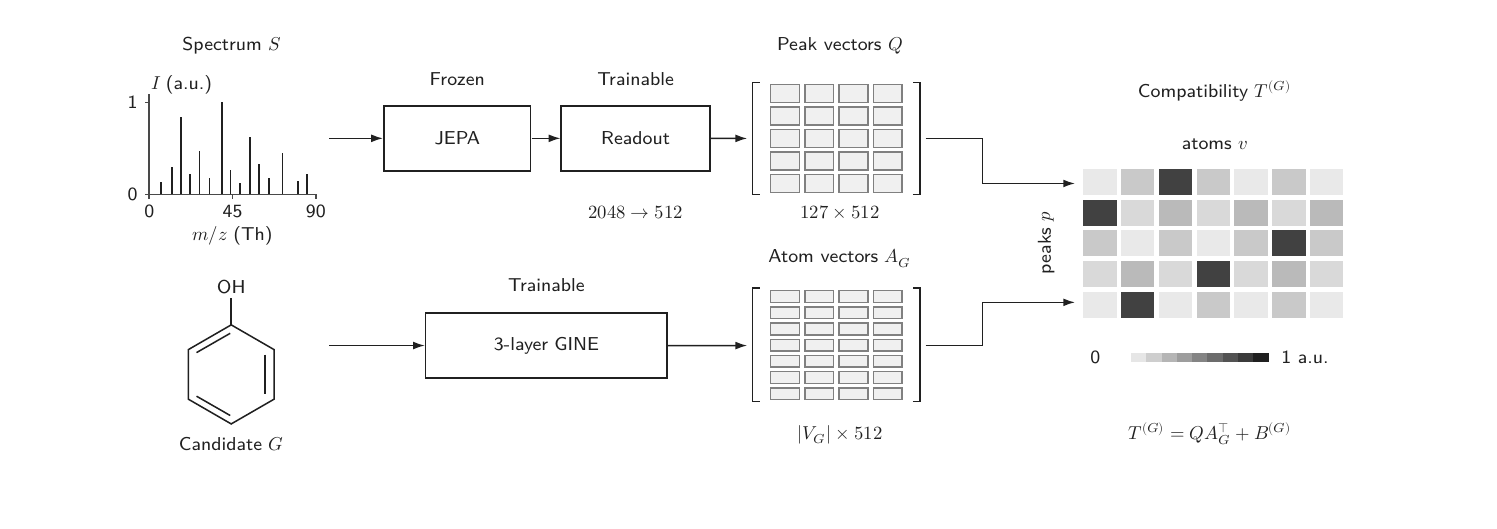
\begin{tikzpicture}[x=1cm,y=1cm,scale=1.14375,transform shape]
% Data are drawn as their scientific objects; boxes denote learned operations.
\node[small] at (2.26,6.65) {Spectrum $S$};
\draw[muted,line width=.55pt] (1.35,5.0)--(3.20,5.0);
\draw[muted,line width=.55pt] (1.35,5.0)--(1.35,6.11);
\foreach \x/\h in {.13/.14,.25/.30,.35/.86,.45/.22,.56/.48,.67/.18,.81/1.02,.90/.27,1.01/.12,1.12/.64,1.22/.34,1.33/.18,1.48/.46,1.65/.15,1.75/.23}{\draw[ink,line width=.55pt] (1.35+\x,5.0)--+(0,\h);}
\foreach \x/\lab in {1.35/0,2.275/45,3.20/90}{\draw[muted,line width=.55pt] (\x,5.0)--+(0,-.055);\node[anchor=north,inner sep=2pt,font=\figurefont] at (\x,4.96) {\lab};}
\foreach \y/\lab in {5.0/0,6.02/1}{\draw[muted,line width=.55pt] (1.35,\y)--+(-.045,0);\node[anchor=east,inner sep=2pt,font=\figurefont] at (1.30,\y) {\lab};}
\node[anchor=west,inner sep=0,font=\figurefont] at (1.36,6.22) {$I$ (a.u.)};
\node[anchor=base,inner sep=0,tinytext] at (2.275,4.49) {$m/z$ (Th)};
\coordinate (specout) at (3.35,5.62);

\node[box,text width=1.35cm,inner xsep=4pt,inner ysep=4pt,minimum height=.72cm] (jepa) at (4.77,5.62) {JEPA};
\node[box,text width=1.37cm,inner xsep=4pt,inner ysep=4pt,minimum height=.72cm] (readout) at (6.75,5.62) {Readout};
\node[small] at (4.77,6.28) {Frozen};
\node[small] at (6.75,6.28) {Trainable};
\draw[arr] (specout)--(jepa.west);
\draw[arr] (jepa.east)--(readout.west);
\node[anchor=base,inner sep=0,small] at (6.75,4.73) {$2048\to512$};

% Each row denotes a feature vector; the cells are coordinate containers.
\node[small] at (9.02,6.65) {Peak vectors $Q$};
\foreach \r in {0,...,4}{\foreach \c in {0,...,3}{\draw[draw=line,fill=soft,line width=.55pt] (8.25+\c*.38,5.02+\r*.25) rectangle +(.32,.20);}}
\draw[ink,line width=.55pt] (8.13,5.00)--(8.05,5.00)--(8.05,6.24)--(8.13,6.24);
\draw[ink,line width=.55pt] (9.83,5.00)--(9.91,5.00)--(9.91,6.24)--(9.83,6.24);
\draw[arr] (readout.east)--(7.99,5.62);
\node[anchor=base,inner sep=0,small] at (9.02,4.73) {$127\times512$};

% A genuine molecular graph depiction (phenol); example is not paired data.
\molecule{2.26}{3.00}{.55}
\node[anchor=base,inner sep=0,small] at (2.26,2.15) {Candidate $G$};
\coordinate (graphout) at (3.35,3.32);
\node[box,text width=2.4cm,inner xsep=4pt,inner ysep=4pt,minimum height=.72cm] (gine) at (5.76,3.32) {3-layer GINE};
\node[small] at (5.76,3.99) {Trainable};
\draw[arr] (graphout)--(gine.west);
\node[small] at (9.02,4.29) {Atom vectors $A_G$};
\foreach \r in {0,...,6}{\foreach \c in {0,...,3}{\draw[draw=line,fill=soft,line width=.55pt] (8.25+\c*.38,2.72+\r*.18) rectangle +(.32,.13);}}
\draw[ink,line width=.55pt] (8.13,2.70)--(8.05,2.70)--(8.05,3.96)--(8.13,3.96);
\draw[ink,line width=.55pt] (9.83,2.70)--(9.91,2.70)--(9.91,3.96)--(9.83,3.96);
\draw[arr] (gine.east)--(7.99,3.32);
\node[anchor=base,inner sep=0,small] at (9.02,2.28) {$|V_G|\times512$};

% Both learned arrays feed a distinct output object.
\draw[arr] (9.97,5.62)--(10.60,5.62)--(10.60,5.12)--(11.63,5.12);
\draw[arr] (9.97,3.32)--(10.60,3.32)--(10.60,3.80)--(11.63,3.80);
\node[small] at (13.18,6.15) {Compatibility $T^{(G)}$};
\node[tinytext] at (13.18,5.55) {atoms $v$};
\node[tinytext,rotate=90] at (11.31,4.46) {peaks $p$};
\foreach \r in {0,...,4}{\foreach \c in {0,...,6}{
 \pgfmathtruncatemacro{\shade}{ifthenelse(mod(2*\r+1,7)==\c,85,10+mod(\r+2*\c,4)*7)}
 \fill[ink!\shade] (11.72+\c*.42,3.63+\r*.34) rectangle +(.37,.29);}}
\foreach \i in {0,...,9}{\pgfmathtruncatemacro{\shade}{\i*100/9}\fill[ink!\shade] (12.08+\i*.17,3.14) rectangle +(.17,.10);}
\node[tinytext,anchor=east,inner sep=2pt] at (11.99,3.19) {0};
\node[tinytext,anchor=west,inner sep=2pt] at (13.84,3.19) {1 a.u.};
\node[anchor=base,inner sep=0,font=\figurefont] at (13.13,2.28) {$T^{(G)}=QA_G^\top+B^{(G)}$};
% Fixed canvas: 183 x 60.046875 mm. No clipping: overflow is audited.
\pgfresetboundingbox
\path[use as bounding box] (0,1.6) rectangle (16,6.85);
\end{tikzpicture}
\end{document}
